\nomenclature[A]{VFM}{Vehicle Following Message}
\nomenclature[A]{PSM}{Platoon Status Message}
\nomenclature[A]{PRR}{Packet Reception Ratio = 100 - PER}
\nomenclature[A]{CSS}{Chirp Signal Spectrum}
\nomenclature[A]{LOS}{Line Of Sight}
\nomenclature[A]{CIRP}{Channel Impulse Response Power}
\nomenclature[A]{PAC}{Preamble Accumulation Count}

In Section 4.1, we define the link quality metrics used for our experimental analysis.
In Section 4.2, we list the set of goals to determine the suitability of using UWB as a secondary independent backup channel for platooning derived from our research questions. In Section 4.3, we explain the role of both the nodes in the network. In Section 4.4, we describe the data communication primitive that will be used to study the link quality. In Section 4.5, we design measurement plans. In Section 4.6, we list the set of requirements of the test platform TP-UWB that enables us to execute the developed measurement plans. In Section 4.7, we list the set of post-processing requirements.

\section{Communication Performance Metrics}
Below we define the various metrics that we use to perform the comparative analysis of different configurations.

\subsection{Packet Error Ratio}
The Packet Error Ratio gives a measure of the relative number of packets lost in a link. We define the following variables:
\begin{itemize}
    \item A = Total number of packets transmitted by the leading truck during the data communication state at the link layer.
    \item B = Total number of packets received by the following truck during the data communication state at the link layer.
    \item C = Total number of packets transmitted by the following truck during the data communication state at the link layer
    \item D = Total number of packets received by the leading truck during the data communication state at the link layer.
    
    We define the packet error ratio (PER) of the leading truck and the following truck using the above variables.
    
    \begin{equation}
    PER_{LeadingTruck} = (C-D)/C
    \label{eq: PERLeadingTruck}
    \end{equation}
    \begin{equation}
    PER_{FollowingTruck} = (A-B)/A
    \label{eq: PERFollowingTruck}
    \end{equation}
    
\end{itemize}

\subsection{Message Error Ratio}
The Message Error Ratio gives a measure of the relative number of messages lost in a link wherein a message is a combination of several packets. We define the following variables:
\begin{itemize}
    \item A = Total number of messages transmitted by the leading truck during data communication state at the application layer.
    \item B = Total number of messages received by the following truck during data communication state at the application layer.
    \item C = Total number of messages transmitted by the following truck during data communication state at the application layer
    \item D = Total number of messages received by the leading truck during data communication state at the application layer.
    
    We define the Message Error Ratio (MER) of the leading truck and the following truck using the above variables.
    
    \begin{equation}
    MER_{LeadingTruck} = (C-D)/C
    \label{eq: MERLeadingTruck}
    \end{equation}
    \begin{equation}
    MER_{FollowingTruck} = (A-B)/A
    \label{eq: MERFollowingTruck}
    \end{equation}
    
\end{itemize}

\subsection{Packet Latency}
It is to be noted that in this thesis, we do not retransmit the packets in the communication state. Hence the message latency and the packet latency provide an indication about the typical latencies involved when this system is integrated with any other system, the number of packets that can be transmitted and received in a given time slot, and an indication about the proper functioning of the system. A message comprises of several packets. Packet latency is the time taken to transfer a packet from the link layer of leading truck to the link layer of following truck or vice versa.
We define the following variables:
\begin{itemize}
    \item Buffer time at the leading truck when transmitting a packet, \emph{$B_{LTX}$}: In the case of a packet sent from the leading truck to the following truck, the time required to copy the payload of a packet to the broadcast packet along with the time taken to write it to the transfer buffer.
    
    \item Buffer time at the leading truck when receiving a packet, \emph{$B_{LRX}$}:  In the case of a packet sent from the following truck to the leading truck, the time required to read the received buffer.
    
    \item Buffer time at the following truck when receiving a packet, \emph{$B_{FRX}$}: In the case of a packet sent from the leading truck to the following truck, the time required to read the received buffer.
    
    \item Buffer time at the following truck when transmitting a packet, \emph{$B_{FTX}$}: In the case of a packet sent from the following truck to the leading truck, the time required to copy the payload of a packet to the broadcast packet along with the time taken to write it to the transfer buffer.
    
    \item Propagation time + Transmission time, \emph{$P_{t}$} = Time taken for a packet to travel from the the leading truck to following truck or vice versa. 
\end{itemize}
As shown in Figure \ref{fig:messageLatencyLeadingtoFollowing} and Figure \ref{fig:messageLatencyFollowingtoLeading}, the packet latency for the leading truck transmitting a packet and following truck transmitting a packet can be calculated using the Equation \ref{eq: packetLatencyLeading} and \ref{eq: packetLatencyFollowing} respectively. 
\begin{equation}
Packet\_Latency_{LTX} = B_{LTX}  +  P_{t} +  B_{FRX}
\label{eq: packetLatencyLeading}
\end{equation}
\begin{equation}
Packet\_Latency_{FTX} = B_{FTX}  +  P_{t} +  B_{LRX}
\label{eq: packetLatencyFollowing}
\end{equation}
\begin{figure}[h!]
	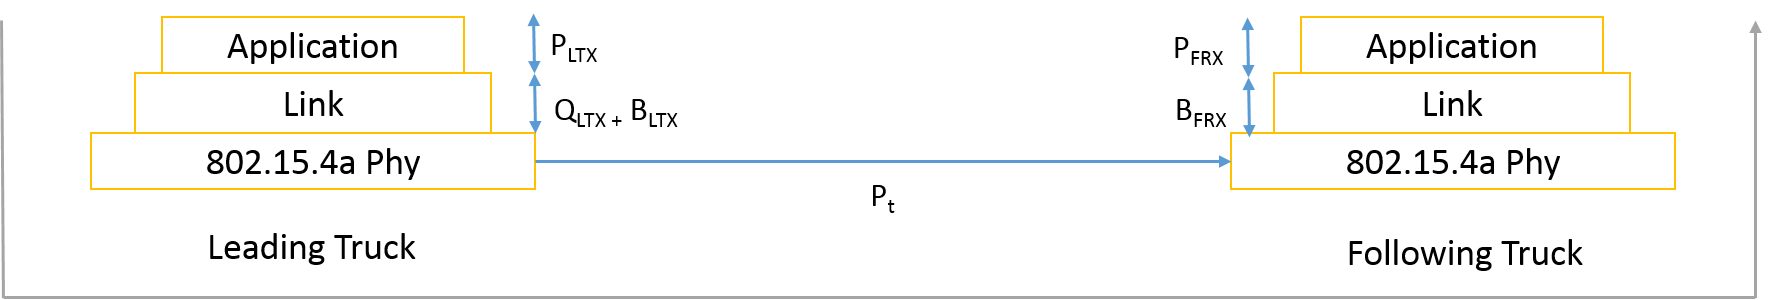
\includegraphics[width=1\textwidth]{figures/messageLatencyLeadingtoFollowing.png}
	\centering
	\caption{End to End latency when a message is transmitted from leading truck to the following truck}
	\label{fig:messageLatencyLeadingtoFollowing}    
\end{figure}
\begin{figure}[h!]
	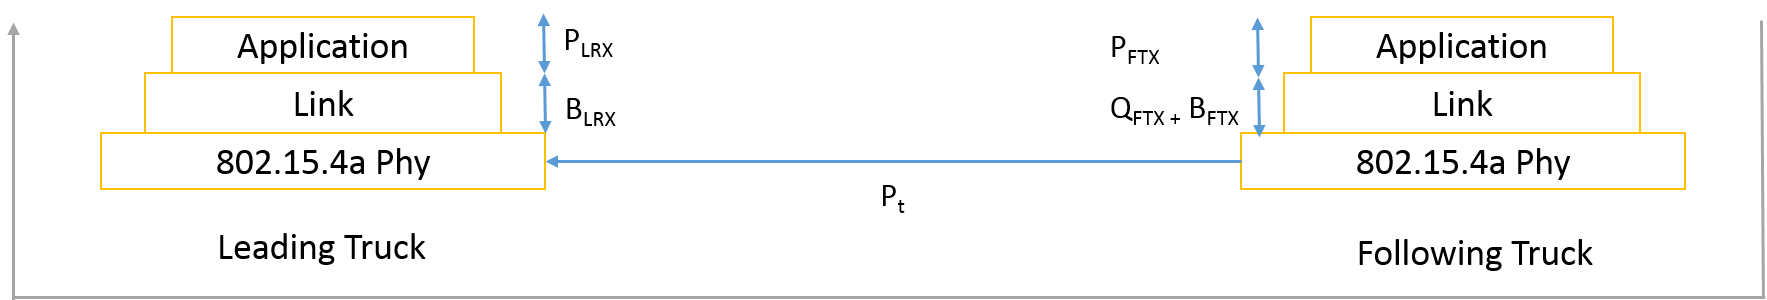
\includegraphics[width=1\textwidth]{figures/messageLatencyFollowingtoLeading.png}
	\centering
	\caption{End to End latency when a message is transmitted from following truck to the leading truck}
	\label{fig:messageLatencyFollowingtoLeading}    
\end{figure}

\subsection{End-to-End Latency/Message Latency}
The end-to-end latency/Message Latency is the time taken for a message to travel from the application layer of the leading truck to the application layer of the following truck or vice versa. We define the following variables:

    \begin{itemize}
    \item Processing time at the leading truck when transmitting a message, \emph{$P_{LTX}$}: In case of a message sent from the leading truck to the following truck,the  time taken to split a message into several packets and push it to the link layer of the leading truck.
    
    \item Processing time at the leading truck when receiving a packet, \emph{$P_{LRX}$}: In the case of a message sent from the following truck to the leading truck, the time taken for the received message to be completely processed by the application layer of the leading truck after the reception interrupt.
    
    \item Queuing time at the leading truck when transmitting a packet, \emph{$Q_{LTX} $}: When packets of a message are transmitted from the leading truck to the following truck, the time spent between transmission of each packet in the link layer of the leading truck.
    
    \item Queuing time at the following truck when transmitting a packet, \emph{$Q_{FTX} $}: When packets of a message are transmitted from the following truck to the leading truck, the time spent between transmissions of each packet in the link layer of the following truck.
    
    \item Processing time at the following truck when transmitting a message, \emph{$P_{FTX}$}:
    In the case of a message sent from the following truck to leading truck, time taken to split a message into several packets and push it to the link layer of the leading truck.
    
    \item Processing time at the following truck when receiving a packet, \emph{$P_{FRX}$}: In the case of a message sent from leading truck to the following truck, the time taken for the received message to be completely processed by the application layer of the following truck after the reception interrupt.
\end{itemize}

As shown in Figure \ref{fig:messageLatencyLeadingtoFollowing} and Figure \ref{fig:messageLatencyFollowingtoLeading}, the end-to-end/message latency for the leading truck transmitting a message and the following truck transmitting a message can be calculated using the Equation \ref{eq: messageLatencyLeading} and \ref{eq: messageLatencyFollowing} respectively wherein No\_of\_packets\_per\_message indicates the number of packets to be transmitted in a message. 
\begin{equation}
Message\_Latency_{LTX} = P_{LTX} + Q_{LTX} + No\_of\_packets\_per\_message * (B_{LTX}  +  P_{t} +  B_{FRX}) + P_{FRX}
\label{eq: messageLatencyLeading}
\end{equation}
\begin{equation}
Message\_Latency_{FTX} = P_{FTX} + Q_{FTX} + No\_of\_packets\_per\_message * (B_{FTX}  +  P_{t} +  B_{LRX}) + P_{LRX}
\label{eq: messageLatencyFollowing}
\end{equation}

\subsection{Reliable and Unreliable link}
We consider the links with MER less than 1\% as a reliable link because we are speaking about a secondary independent channel, wherein a loss of ten message for every thousand messages is acceptable for platooning.

\section{Measurement Goals}
To answer each of our research questions introduced in Section 1.4, we design a set of measurement goals corresponding to each question.

\subsection{Research Question RQ\_01}
What is the impact on the performance (Packet Error Ratio, Message Error Ratio, message latency, packet latency) of UWB in the presence of WiFi-p and vice-versa?

\subsubsection{Measurement Goal MG\_Interference}
In the measurement goal MG\_Interference, we investigate the performance of the UWB link in the presence of WiFi-p and vice versa based on link quality metrics PER, MER, message latency, and packet latency. Besides, we investigate the effect of Channel, Preamble Length, PRF (Pulse Repetition Frequency), Standard SFD, Non-standard SFD, Smart Power enablement, Preamble code on the performance of the UWB link in the presence of interference.

\subsubsection{Measurement Goal MG\_Distance\_Between\_Transceivers}
In the measurement goal MG\_Distance\_Between\_Transceivers, we study the influence of distance between UWB transceiver and WiFi-p transceiver on the links based on link quality metrics.


\subsubsection{Measurement Goal MG\_Worst\_Case\_Interference}
In the measurement goal MG\_Worst\_Case\_Interference, we investigate the performance of UWB link in the presence of WiFi-p and vice versa, by maximizing the time domain overlap of transmission instants, based on link quality metrics.

\subsection{Research Question RQ\_02}
Sensitivity analysis of performance under various conditions:

\subsubsection{Measurement Goal MG\_Speed\_Or\_Acceleration\_Difference}
In the measurement goal MG\_Speed\_Or\_Acceleration\_Difference, we investigate the performance of UWB link in the presence of speed or acceleration difference, based on link quality metrics.

\subsubsection{Measurement Goal MG\_Nulls}
In the measurement goal MG\_Nulls, we investigate the performance of UWB link at a distance of 20-30 m, based on link quality metrics. A null could arise because of negative interference from different multipaths. If the Line Of Sight (LOS) signal and the multipath signal, arrive at the destination at the same instant of time, negative interference could lead to no signal being received resulting in a null.

\subsection{Research Question RQ\_03}
What is the ranging accuracy that can be achieved through UWB when the trucks are operating in platooning mode?

\subsubsection{Measurement Goal MG\_Ranging\_Accuracy}
In the measurement goal MG\_Ranging\_Accuracy, we investigate the static ranging accuracy that can be achieved through UWB based on the difference between calculated distance and actual distance. Besides, we also examine the effect of Standard SFD and Non-Standard SFD on ranging accuracy.

\subsection{Research Question RQ\_04}
Which is the best configuration of UWB for platooning application?

Analyzing all the results, we determine the best configuration of UWB for platooning application.

\section{Network Topology}
We use point to point topology (Figure: \ref{fig:NetworkTopology}), wherein we have two nodes, namely the leading truck and the following truck. We use point to point topology as we consider platooning between two trucks as the situation under test and the existing EcoTwin Platooning project (project collaboratively developed by NXP, DAF Trucks and TNO) operates on the same topology \cite{euTPC}.

Below we describe the functions of each component present in our network topology (shown in Figure: \ref{fig:NetworkTopology}):

\begin{itemize}
    \item \textbf{Leading Truck}: In the communication state, the Vehicle Following Message (VFM) is sent from the leading truck to the following truck every 40 milliseconds starting from the instant of 0 millisecond. Also, it receives the Platoon Status Message (PSM) from the following truck. The node is an LPCXpresso 4337 board with DecaWave DW1000 transceiver.
    \item \textbf{Following Truck}: In the communication state, the PSM is sent from the following truck to the leading truck every 40 milliseconds starting from the instant of 20 milliseconds. Also, it receives the VFM from the leading truck. The node is an LPCXpresso 4337 board with DecaWave DW1000 transceiver.
    \item \textbf{Laptop/PC}: Laptop/PC is used as the human interface to log the data exported by the leading truck via the serial interface. The leading truck is interfaced to a laptop/PC through a USB port.
\end{itemize}

\begin{figure}[h!]
    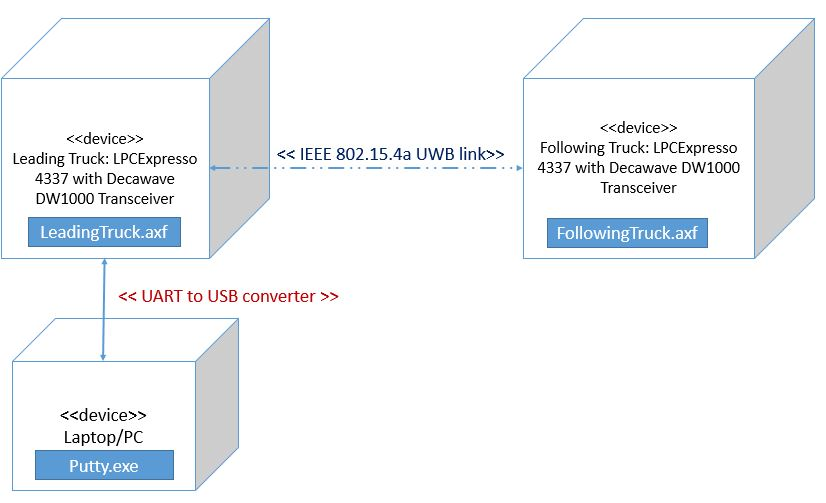
\includegraphics[width=1\textwidth]{figures/networkTopologyDeployment.JPG}
    \centering
    \caption{Point to Point topology deployment diagram}
    \label{fig:NetworkTopology}    
\end{figure}

\section{Data Communication Primitive}
We consider the data communication primitive to quantify the link characteristics in both directions: i. Uplink: leading truck to the following truck, and ii. Downlink: following truck to the leading truck.

    \textbf{Data Communication}: In the case of data communication state, VFM is sent from leading truck to the following truck every 40 milliseconds starting from the instant of 0 millisecond, PSM is sent from the following truck to leading truck every 40 milliseconds starting from the instant of 20 milliseconds. This communication primitive is designed to mimic the actual exchange of messages that occurs during platooning as shown in Figure \ref{fig:MessageExchangePlatooningApplication}.
    
    \begin{figure}[htbp]
        \begin{center}
            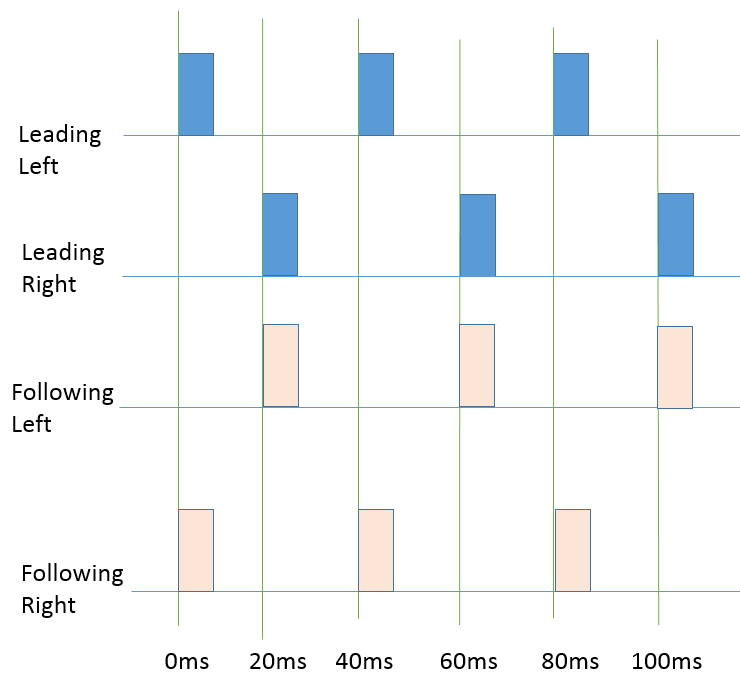
\includegraphics[width=0.8\textwidth]{figures/Picture6.png}
            \caption{Message Exchange in Platooning Application}
            \label{fig:MessageExchangePlatooningApplication}
        \end{center}
    \end{figure}

\section{Measurement Plan}
The measurement goals defined in Section 4.2 necessitate the need for varying different parameters such as packets per message, channels, PRF, preamble lengths, preamble codes, Standard or non-standard SFD, Smart Power enablement, distance, speed or acceleration, etc. to study their influence on the link quality. We design three measurement plans, to explore these measurement goals by sweeping a parameter over a range of values while keeping the other parameters constant. We use the measurement plan as a tool to perform experiments with/without vehicles and on the table top. Below we describe the measurement plans in detail.

\subsection{Measurement Plan MP\_Interference}
In measurement plan MP\_Interference, we investigate the performance of UWB in the presence of WiFi-p and vice versa based on link quality metrics. This measurement plan helps us to study measurement goals MG\_Interference, MG\_Distance\_Between\_Transceivers, and MG\_Worst\_Case\_Interference.

To introduce WiFi-p signals, we use equipment from Cohda wireless. Python scripts are used to monitor the sent and received messages. We operate WiFi-p in channel 184 corresponding to 5.920 GHz so that we get closest to channel 7 of UWB.

UWB transceivers are placed at an appropriate distance (0cm and 80cm) to the WiFi-p antennas, and we sweep several parameters as shown in Table \ref{configurationsMPInterference}. UWB transceiver - leading truck transmits every 40 ms starting at the 0 ms instant, and the UWB transceiver - following truck transmits every 40 ms starting at the 20 ms instant. We run a total of 44 configurations (\ref{app:ConfigurationsforMeasurementPlanMPInterference}) in this measurement plan varying several parameters as indicated in the Table \ref{configurationsMPInterference}.
% Please add the following required packages to your document preamble:
% \usepackage{graphicx}
\begin{table}[]
    \centering
    \caption{Configurations for measurement plan MP\_Interference}
    \label{configurationsMPInterference}
    \resizebox{\textwidth}{!}{%
        \begin{tabular}{|l|l|}
            \hline
            \textbf{Sweep Parameter}                            & \textbf{Value}                                \\ \hline
            Channels                                            & Channel 1, Channel 3, Channel 5 and Channel 7 \\ \hline
            PRF                                                 & 16Mhz and 64 MHz                              \\ \hline
            Data Rate                                           & 6.8 Mbps                                      \\ \hline
            Preamble Lengths                                    & 256, 128 and 64                               \\ \hline
            SFD                                                 & Standard or Non-Standard SFD                  \\ \hline
            Distance between WiFi-p antenna and UWB transceiver & 80 cm and 0 cm                                \\ \hline
            Smart Power Enablement                              & With and Without Smart Power Enablement       \\ \hline
            Preamble Code                                       & According to the Channel                      \\ \hline
        \end{tabular}%
    }
    
\end{table}

We conduct this measurement plan keeping the distance between UWB transceivers and WiFi-p Antenna at 80 cm and 0 cm to evaluate measurement goal MG\_Distance\_Between\_Transceivers. To assess MG\_Worst\_Case\_Interference, we transmit as quickly as possible (one message every 8 ms) from the UWB transceiver-leading truck and receive them at the UWB transceiver-following truck without adhering to the 40 ms constraint, so that we increase the time domain overlap between WiFi-p transmission and UWB transmission. 

\subsection{Measurement Plan MP\_Speed\_Or\_Acceleration\_Difference}
In measurement plan MP\_Speed\_Or\_Acceleration\_Difference, we mount the UWB transceivers on the mirrors of two cars. We make static measurements, following which we move one of the cars at 5-15 Km/hr to determine the influence of speed or acceleration difference on the performance of UWB link based on the link quality metrics. In this measurement plan, we vary parameters according to Table \ref{table:configurationsformeasurementplanMPSpeedDifference}. To overcome the major drawback of short range when using 6.8 Mbps data rate, we make use of 110 Kbps as the data rate in this measurement plan. This measurement plan helps us to study the measurement goals MG\_Nulls and MG\_Speed\_Or\_Acceleration\_Difference. 

% Please add the following required packages to your document preamble:
% \usepackage{graphicx}
\begin{table}[]
    \centering
    \caption{Configurations for measurement plan MP\_Speed\_Or\_Acceleration\_Difference}
    \label{table:configurationsformeasurementplanMPSpeedDifference}
    \begin{tabular}{|l|l|}
        \hline
        \textbf{Sweep Parameter} & \textbf{Value}               \\ \hline
        Channel                  & Channel 1                    \\ \hline
        PRF                      & 64 MHz                       \\ \hline
        Data Rate                & 110 Kbps                     \\ \hline
        Preamble Lengths         & 2048, 4096                   \\ \hline
        SFD                      & Standard or Non-Standard SFD \\ \hline
        Preamble Code            & According to the Channel     \\ \hline
    \end{tabular}
\end{table}


\subsection{Measurement Plan MP\_Distance}
In measurement plan MP\_Distance, we investigate the influence of distance on UWB link, based on the link quality metrics. Here, we keep the UWB transceivers at various distances and measure the link quality. In this measurement plan, we vary parameters according to the Table \ref{tab:configurationsforMPDistance}. This measurement plan helps us to study the measurement goals MG\_Ranging\_Accuracy and MG\_Nulls. We also determine the effect of antenna position on the link quality.

\begin{table}[]
    \centering
    \caption{Configurations for measurement plan MP\_Distance}
    \label{tab:configurationsforMPDistance}
    \begin{tabular}{|l|l|}
        \hline
        \textbf{Sweep Parameter} & \textbf{Value}                               \\ \hline
        Channel                  & Channel 1, Channel 4                         \\ \hline
        PRF                      & 16 MHz, 64 MHz                               \\ \hline
        Smart Power              & Enabled or Not Enabled                       \\ \hline
        Data Rate                & 110 Kbps, 850 Kbps, 6.8 Mbps                 \\ \hline
        Preamble Lengths         & 2048, 4096, 1024, 256                        \\ \hline
        SFD                      & Standard or Non-Standard SFD                 \\ \hline
        Preamble Code            & According to the Channel                     \\ \hline
        Antenna Position         & 0, 45, 90, 135, 180, 225, 270, 315 (degrees) \\ \hline
        Distance                 & 10, 15, 20, 25, 30, 35, 40, 45, 50 (meters)  \\ \hline
    \end{tabular}
\end{table}
\section{Test Platform Requirements}

The test platform implements the necessary functionalities to execute the measurement plans discussed in Section 4.5. Based on our measurement plans and measurement goals defined in the previous Sections, we develop the following set of requirements for our test platform.

\begin{enumerate}
    \item It must support point to point topology with one transceiver-leading truck and another transceiver-following truck. 
    \item It must implement data communication workload and transmit/receive according to the 40 ms schedule.
    \item It must enable us to vary parameters such as packets per message, channels, PRF, preamble lengths, preamble codes, Standard or non-standard SFD and Smart Power enablement.
    \item It must capture physical layer metrics such as Channel Impulse Response Power (CIRP), Preamble Accumulation Count (PAC), accurate time stamps for ranging, and sequence numbers of the test payload, at both transceivers.
    \item It must enable the following truck to store the logging information and communicate this information to the leading truck.
    \item It must allow the transceivers to send the logging information and print the log via the serial interface connection to the laptop/PC.
    \item It should run autonomously without human intervention and execute all possible test combinations of parameters based on the selected measurement plan so that the manual effort required for the same can be significantly reduced.
\end{enumerate}

\section{Post Processing Requirements}
The task of the post-processing scripts is to parse and extract useful information from the logs created during the experiments.

For the post processing we have the following requirements:
\begin{enumerate}
    \item It must be able to process logs resulting from a full night test.
    \item It should parse the log files and store the data appropriately so that desired kind of graphs such as PER vs. Channel, MER vs. Channel, MER vs. Distance, Measured Distance vs. Calculated Distance, etc. can be created.
\end{enumerate}